% APÊNDICES--------------------------------------------------------------------

\begin{apendicesenv}
\partapendices

% Primeiro apêndice------------------------------------------------------------
\chapter{Opinião: Guilherme Cosso} % Edite para alterar o título deste apêndice
\label{chap:apendiceA}

O que mais me chamou a atenção na linguagem tema Python foi a sua nomenclatura baseada no seriado Monty Python.
O seu criador Guildo Van Russo queria uma linguagem forte para a LP.
Apesar de todos associarem a Lp as cobras pithón.
As trocas de variáveis sem conter uma terceira para fazer a troca, além de não ser necessário ponto e virgula "$;$" , chaves "\{" e a Main como pode ser visto abaixo:

\begin{figure}[!htb]
    \centering
    \caption{Exemplo de Código}
    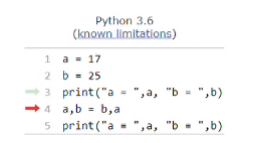
\includegraphics[width=0.5\textwidth]{./dados/figuras/cosso1.png}
    \fonte{Original}
    \label{fig:figura-mountPython}
\end{figure}

A tipagem fraca e o seu conteúdo ser dinamicamente tipada: o tipo de conteúdo de variável poder mudar automaticamente.

\begin{figure}[!htb]
    \centering
    \caption{Exemplo de Tipagem}
    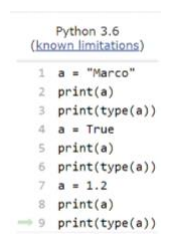
\includegraphics[width=0.35\textwidth]{./dados/figuras/cossin2.png}
    \fonte{Original}
    \label{fig:figura-mountPython}
\end{figure}

% Novo apêndice----------------------------------------------------------------
\chapter{Opinião: Iyan Lucas}
\label{chap:apendiceB}

Recentemente, comecei a exercer minha iniciação científica sob o Observatório da Saúde. 
Comecei a gostar de séries temporais e, apesar do meu apreço por linguagens como Java, C\# e C++, Python era essencial para tudo, desde a análise de dados à plotar pontos em mapas.
Fui, entre muitas áspas, "forçado" ao aprendizado da linguagem. 
Percebi de imediato, a minha estranheza com a falta de ponto-e-vírgula e chaves, sobretudo a ausência de uma main.
\par Agora, ao redigir este apêndice, estou bem acostumado ao Python, programando todo dia, todo meses com a linguagem e então me realizei da grandeza da LP.
Ela é, apesar de confusa, funcional, curta, simples e prática.
Fiquei assustado pela eficiência dela com grandes bases de dados e rapidez.
Apesar de que eu penso que faria os programas mais organizados e mais intuitivamente em Java, percebi que essa visão minha é só um ponto de vista de muitos.

\chapter{Opinião: Samir Cambraia}
\label{chap:apendiceB}

Depois da pesquisa, minha visão sobre a linguagem ficou mais abrangente.
Python é uma linguagem promissora com um grande currículo em aplicações em diversas áreas sendo a mais competente em em sua maioria, tendo sua simplicidade no aprendizado a programação possibilitando o conhecimento de rápida teoria/prática.
\par Porém, na minha opinião as estruturas e regras que levam a grande possibilidade de grandes códigos serem executados com menos trabalho e "linhas" é que me incomoda pelo fato de, como em java, se ter um controle maior e não esperar que a linguagem em si possibilite sem saber o que ocorre por trás assim pessoas com novas experiências, na minha opinião, ficaria rasas em conhecimento como na parte de memória e outros conhecimentos conquistados em linguagens de baixo nível que possibilitam maior controle.


\end{apendicesenv}
